\chapter[Conjunto de dados]{Conjunto de dados}

Os currículos Lattes estão disponíveis online em formato PDF, HTML e XML. Entretanto, a coleta em lotes só é possível para projetos específicos, após obterem a permissão apropriada \cite{medeiros2013dynamics}.

Apesar disso, como mostram \citeonline{mena2009scriptlattes}, a coleta dos currículos pode ser feita com o uso de ferramentas que exploram cada currículo individualmente. O problema, entretanto, está no fato de que o custo computacional para obter os milhões de currículos disponíveis na plataforma um a um é bastante alto. Por esse motivo, o escopo foi limitado a todos os pesquisadores com nível de formação acadêmica igual ou acima de doutorado.

O Grupo de Pesquisa em Cientometria do CMCC/UFABC realizou em janeiro de 2019 a coleta dos currículos no formato XML que foram considerados neste trabalho. Nas seções seguintes são apresentadas informações relativas a esse conjunto de dados.

\section{Análise dos metadados}

Foram obtidos $315.155$ currículos, dos quais $29$ estavam corrompidos e $723$ apresentavam um aviso de erro no conteúdo do arquivo, resultando em $314.403$ currículos válidos. Para se ter uma ideia do volume de dados, são $113$ gigabytes de arquivos no formato XML contendo mais de $2,8$ bilhões de atributos e $569$ milhões de elementos.

Sabendo que os dados não têm preenchimento obrigatório, foi realizado um estudo para conhecer como cada um dos campos estava populado no conjunto de dados. Isso permitiria entender a viabilidade de se considerar uma característica do currículo do pesquisador.

Informações sobre as áreas de atuação e produção bibliográfica estão presentes em $95\%$ e $94\%$ dos currículos, respectivamente. As produções técnicas também estão presentes em grande parte dos currículos, são ao todo $275.361$ currículos com essa informação preenchida. A \autoref{tab:metadadosproducaobibliografica} apresenta quanto cada um dos tipos de produção bibliográfica está presente nos currículos. 

\begin{table}[htpb]
    \centering
    \caption{Frequência do tipo de produção bibliográfica por currículo.}
    \label{tab:metadadosproducaobibliografica}
    \begin{tabular}{|r|l|c|}%
        \hline & Tipo de produção bibliográfica & Número de currículos \\\hline
        \csvreader[late after line=\\\hline]%
        {"tabelas/conjuntodedados-producao-bibliografica.csv"}%
        {no=\no,contagem=\contagem}%
        {\thecsvrow & \no & \contagem}%
    \end{tabular}
\end{table}

Avaliando como os níveis de formação acadêmica estão cadastrados nos currículos, foi possível observar que muitos preenchem dados sobre a graduação e mestrado, como apresenta a \autoref{tab:formacaoacademica}, sendo que bastaria cadastrar o doutorado ou nível acima, o que sugere que todo o histórico de formação acadêmica é preenchido pelos pesquisadores.

\begin{table}[htpb]
    \centering
    \caption{Frequência dos níveis de formação acadêmica por currículos.}
    \label{tab:formacaoacademica}
    \begin{tabular}{|r|l|c|}%
        \hline & Nível de formação acadêmica & Número de currículos \\\hline
        \csvreader[late after line=\\\hline]%
        {"tabelas/conjuntodedados-nivel-de-formacao.csv"}%
        {no=\no,contagem=\contagem}%
        {\thecsvrow & \no & \contagem}%
    \end{tabular}
\end{table}

A partir desse estudo, também foi possível construir os diagramas apresentados no \autoref{ap:diagramacurriculo}, que ajudam a entender a estrutura do currículo, e uma especificação formal do currículo no formato XSD\footnote{O XML Schema Definition (XSD) é uma especificação que descreve os elementos e atributos que um determinado arquivo XML pode conter.}, a qual pode ser usada para a definição da estrutura do banco de dados. Vale observar a especificação oficial dos currículos\footnote{A especificação oficial do currículo Lattes no formato DTD está disponível em \url{http://lattes.cnpq.br/web/plataforma-lattes/extracao-de-dados}.} está no formato DTD, um padrão que vem sendo substituído desde 2009 e costuma não ser suportado por ferramentas e bibliotecas de interpretação de arquivos XML mais recentes.

Com isso, foi considerado a construção de um banco de dados que abrangesse todas as informações relevantes do currículo. Assim, uma vez que as coautorias estivessem identificadas, seria possível explorar métricas considerando não só as áreas de atuação do pesquisador, mas também outras características, como o histórico de formação acadêmica, linha de pesquisa, atuação profissional, produção técnica, dentre outras.

Contudo, não foram encontrados meios que suprissem as necessidades técnicas impostas por um banco de dados desta magnitude\footnote{
Devido ao volume de dados e tempo necessário, não seria possível realizar o processamento em um computador pessoal. Assim, no início, um servidor privado de um professor da Universidade Federal de Mato Grosso do Sul (UFMS) foi utilizado, mas a colaboração foi terminada após alguns meses. Depois disso, dois grandes provedores de nuvem foram contatados, mas ambos não ofereciam os recursos necessários em seus planos dedicados a estudantes.}. Assim, para viabilizar a construção das redes de coautoria e colaboração entre as áreas, o conjunto de dados ficou limitado às áreas de atuação do pesquisador e aos tipos de produção bibliográfica com maior número de ocorrências: publicações em periódicos, publicações em eventos, livros e capítulos de livro.

\section{Características do conjunto de dados}

Os currículos contemplam publicações em periódicos e publicações em evento que podem ter diferentes naturezas: resumo, resumo expandido, publicação completa ou não especificado. Ainda, apesar dos capítulos de livro serem sempre de livros publicados, os livros podem tanto se referir aos publicados quanto aos organizados.

Neste trabalho são consideradas apenas publicações completas em periódicos, publicações completas em eventos, livros publicados e capítulos de livros publicados, as quais são referenciadas como publicações científicas. Foram extraídas $9.968.877$ publicações científicas dos $314.403$ currículos avaliados, e caso todas as naturezas fossem consideradas esse número chegaria a $17.526.806$, como mostra a \autoref{tab:publicacoescientificas}.

\begin{table}[htpb]
    \centering
    \caption{Número de publicações científicas e número considerando todas as naturezas das publicações por tipo de publicação.}
    \label{tab:publicacoescientificas}
    \begin{tabular}{|l|r|r|}%
        \hline & Publicações científicas & Todas as naturezas \\ \hline
        \csvreader[late after line=\\\hline]%
        {"tabelas/conjuntodedados-publicacoes-cientificas.csv"}%
        {tipo=\tipo,filtrado=\filtrado,total=\total}%
        {\tipo & \filtrado & \total}%
    \end{tabular}
\end{table}

Depois do título, o ano de publicação é o campo mais importante para o método desenvolvido. Por isso, é importante que esteja corretamente preenchido. No conjunto das publicações científicas são apenas $914$ casos onde o campo está sem valor válido, o que representa menos de $0,0001$\% dos casos.

O número de autores, isto é, pesquisadores que escreveram alguma publicação científica, é de $290.927$, de um total de $314.403$ pesquisadores. Desses, $238.585$ escreveram publicações em coautoria, o que significa que a vasta maioria dos autores também é realiza coautor. O número de coautores que colaboraram com pesquisadores de outras áreas é de $199.357$, o que reforça a ideia de que a ciência é colaborativa.

São $288.730$ os pesquisadores que cadastraram suas áreas de atuação além da grande área do conhecimento. A maioria declara que atua em apenas uma área do conhecimento, como mostra o gráfico da \autoref{fig:areasdeatuacaodistintas}.

\begin{figure}[htpb]
  \centering
  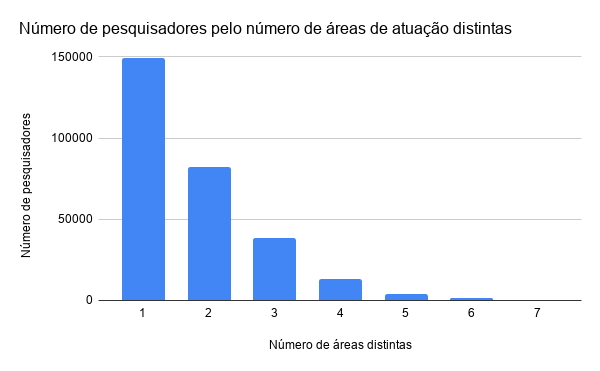
\includegraphics[width=.8\textwidth]{figuras/conjuntodedados-numero-de-areas-distintas}
  \caption{Histograma do número de pesquisadores pelo número de áreas de atuação distintas.}
  \label{fig:areasdeatuacaodistintas}
\end{figure}
